\chapter{Partikelfysik}

\section{Standardmodellen}
Standardmodellen er som navnet antyder den model fysikkere verden over betragter som vores bedste bud på hvordan verden fungerer på sit mest grundlæggende plan. For at beskrive hvordan verdens mindste bestanddele fungerer, skal man kunne beskrive alle typer af vekselvirkninger eller kræfter: Elektromagnetisme, den svage kernekraft, den stærke kernekræft og gravitation. Standardmodellen er elektromagnetisme og de to kernekræfter udtrykt i det der hedder kvantefeltteori, men det er endnu ikke lykkedes at forene disse tre kræfter med tyngdekraften beskrevet af Einsteins generelle relativitetsteori. Dette tyder på at der må eksistere en bedre teori end standardmodellen, og selvom der eksisterer mange bud, har alle disse bud store problemer, hvorfor standardmodellen er vores indtil videre bedste bud. Standardmodellen beskriver verden som bestående af en række elementarpartikler, der kan kombineres til en hel zoologisk have af partikler ligesom legoklodser kan kombineres til store og små konstruktioner. For at holde styr på medlemmerne af denne zoologiske have opdeles partiklerne i grupper efter deres egenskaber. I første omgang inddeles partikler i to store grupper, der henholdvis hedder bosoner, opkaldt efter Satyendra Nath Bose, og fermioner opkaldt efter Enrico Fermi. Fermioner defineres som partikler med halvtalligt spin, det vil sige at $S_\mathrm{fermion} \in \{1/2,3/2,5/2,...\}$, mens bosoner har heltalligt spin, altså $S_\mathrm{boson} \in \{1,2,3,...\}$. Den store vigtighed i disse opdeling ligger i selve den matematik, der beskriver hvordan partiklerne opfører sig, hvilket ikke beskrives her. Spin er en fundamental egenskab ved elementarpartikler, der matematisk opfører sig som om elementarpartiklerne drejer rundt som en snurretop. Det er dog kun den matematiske beskrivelse, der er den samme, for en rotation kan stoppes, hvis man skyder to partikler imod hinanden på den rigtige måde - det kan spin ikke. Der eksisterer derfor ikke nogen god analogi for hvad spin egentligt er, og det betragtes som en egenskab ved en partikel på lige fod med dens elektriske ladning eller dens masse. Et resultat af denne matematik er at fermioner opfylder det der hedder Paulis udelukkelsesprincip, som siger at \emph{to fermioner ikke kan befinde sig i samme kvantetilstand}. Et eksempel på Pauliprincippet er elektroner i atomer fordeller sig i forskellige skaller og ikke blot samler sig i den skal med mindst energi, hvilket er forbudt idet elektroner har spin $S_\mathrm{elektron} = 1/2$, hvorfor de er fermioner. Da standardmodellen indeholder 30 elementarpartikler, er det smarte at opskrive et skema, som kan hjælpe med at give et overblik over alle partiklerne. Et sådant skema er vist i figur \ref{fig:standardmodellen}, og det er en rigtig god ide at konsultere dette skema, mens de forskellige partikler i standardmodellen gennemgås nedenfor.

\begin{figure}
    \centering
    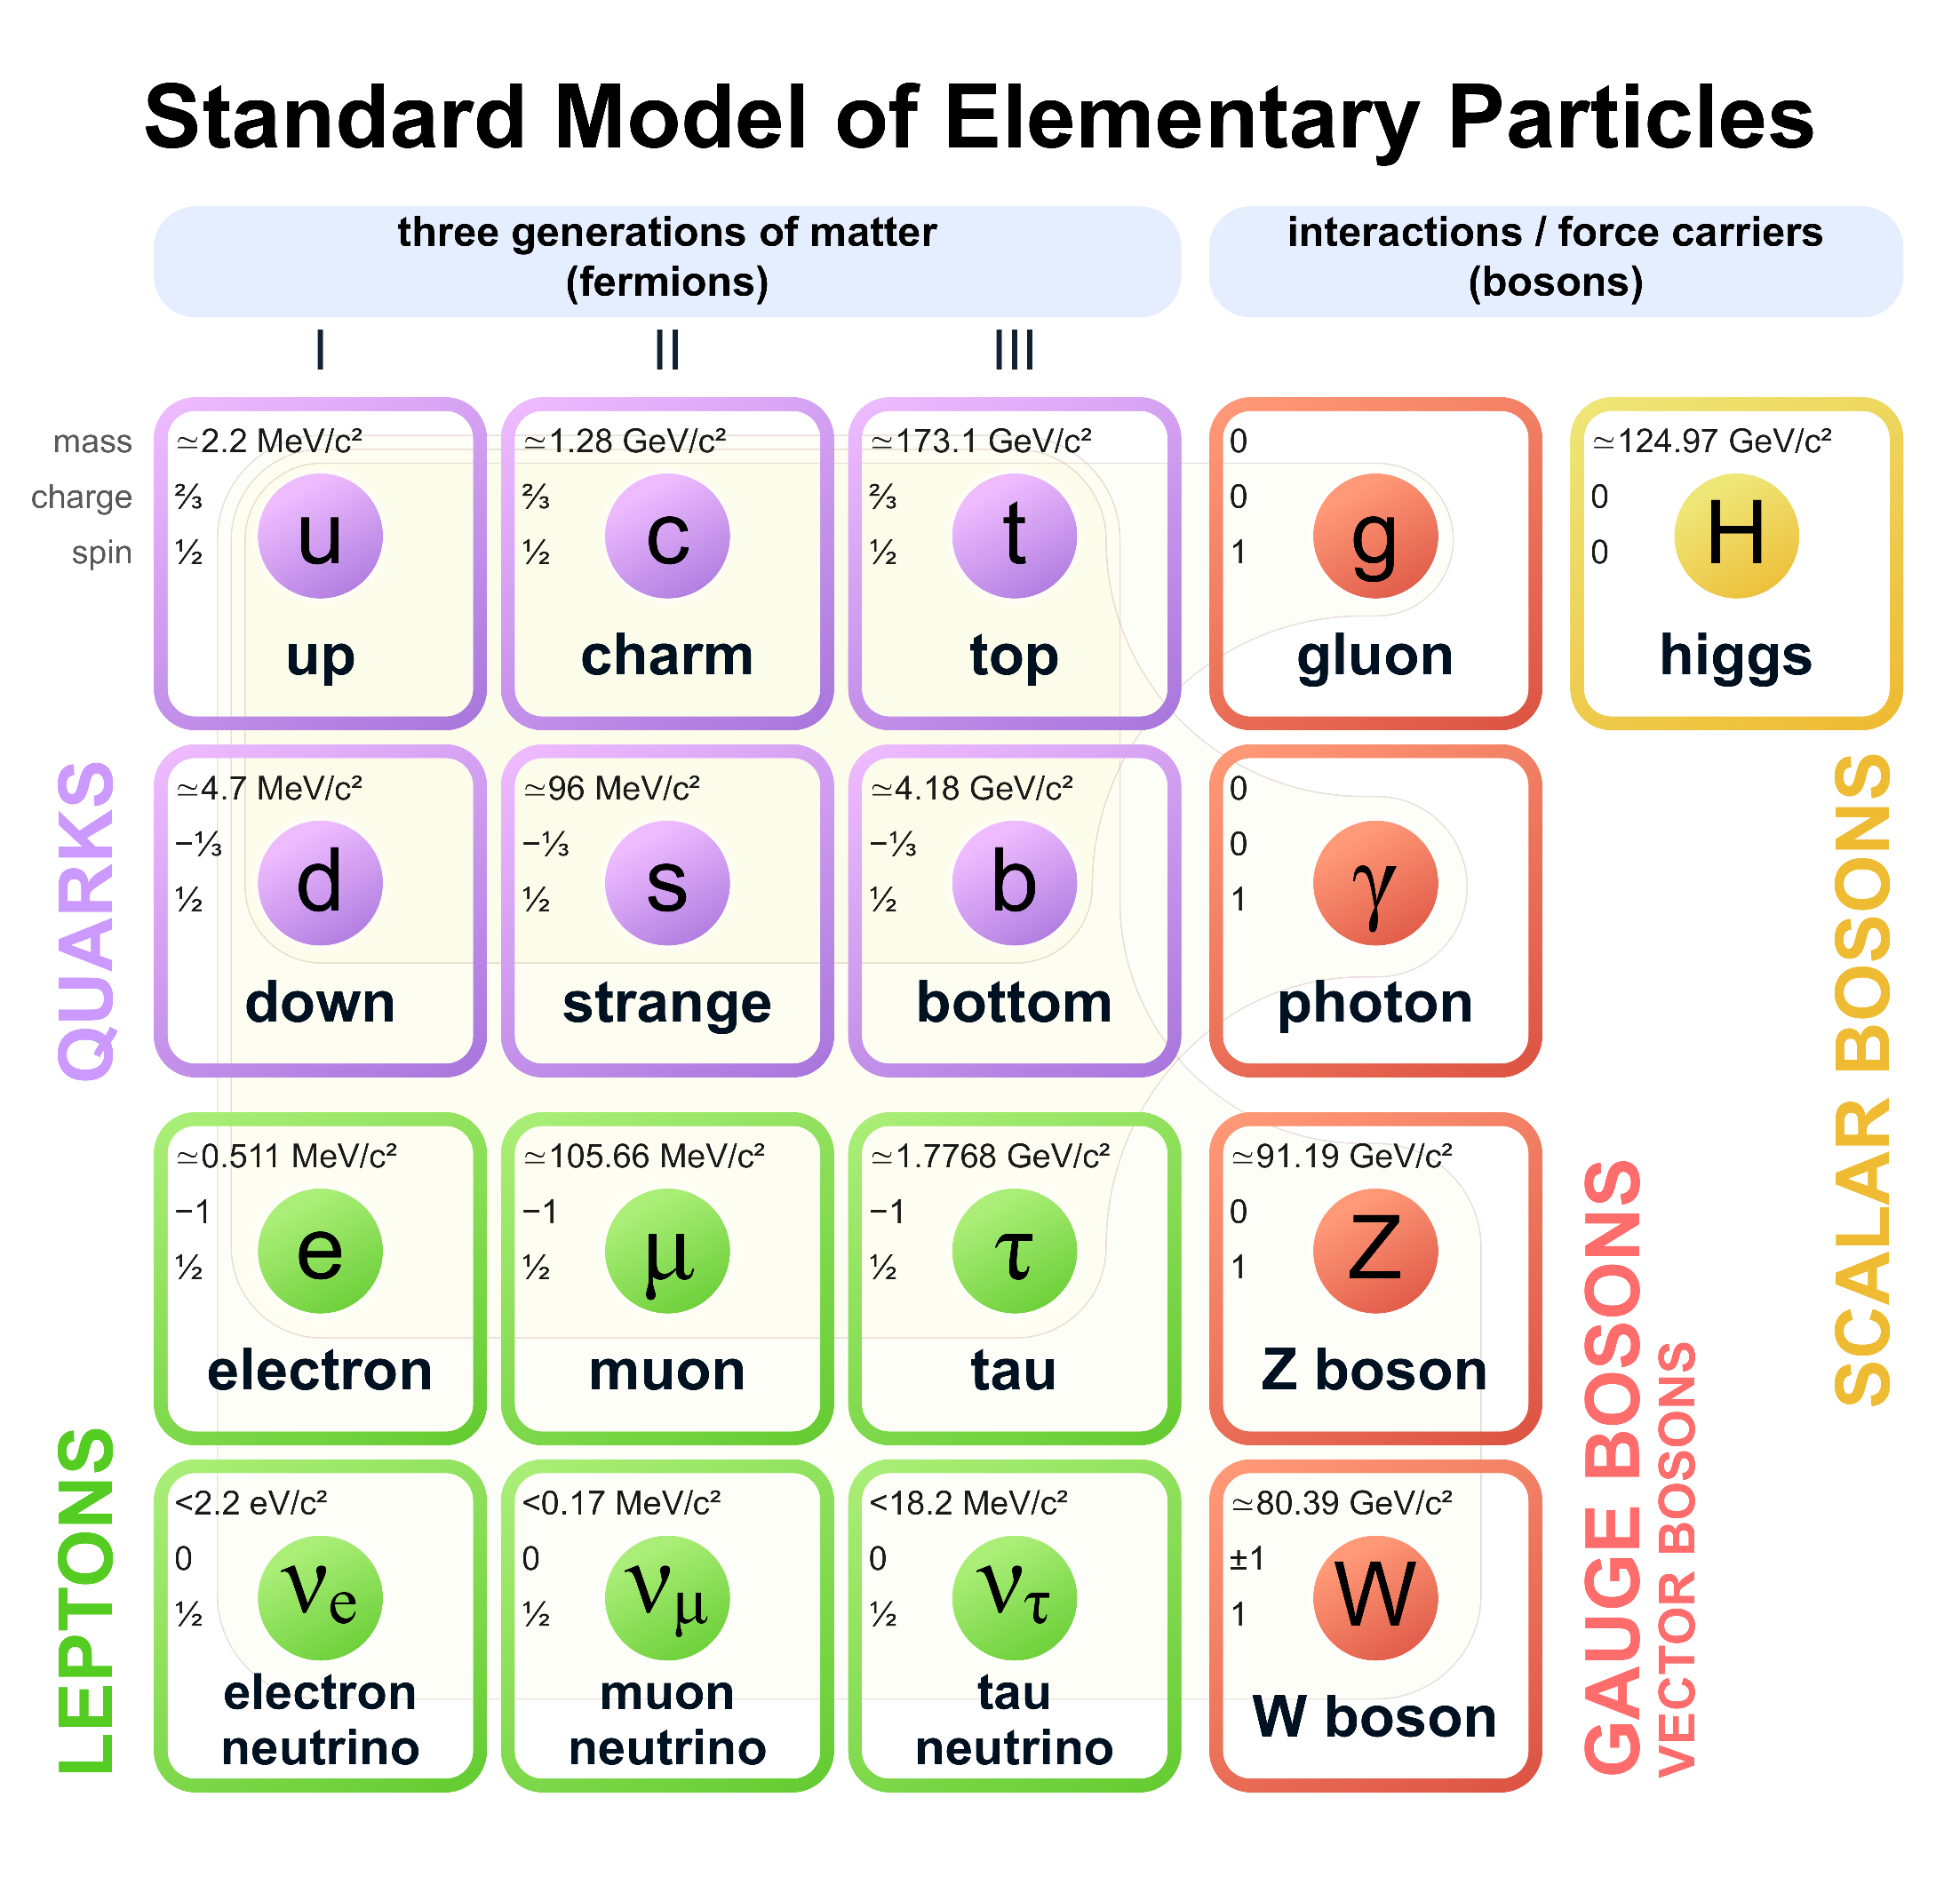
\includegraphics[width=.75\textwidth]{Partikel/figurer/standardmodellen.eps}
    \caption{Skematisk opstilling af elementarpartiklerne, hvor deres masse, elektriske ladning og spin fremgår, samt hvilket gruppe hver partikel tilhører.}
    \label{fig:standardmodellen}
\end{figure}

\subsection{Fermioner}
Fermioner opdeles i to grupper - leptoner og kvarker efter om de har det man kalder farveladning eller sagt på en anden måde om de er påvirket af den stærke kernekraft. I kapitel \ref{sec:ladning} blev konceptet om elektrisk ladning introduceret og i resten af kapitel \ref{chap:el} blev ideen om elektriske og magnetiske felter udforsket samt hvordan ladede partikler vekselvirker med disse. Mere specifikt viser ligningerne \ref{eq:e-felt_punktpartikel} og \ref{eq:kraft_fra_e-felt} at det elektriske felt fra en partikel er proportionalt med partiklens ladning, $\va E \propto q$ og at kraften et elektrisk felt påvirker en partikel med også er proportional med ladningen $\va E \propto q$. Den elektriske ladning kan derfor forstås som et tal, der fortæller hvor meget en partikel vekselvirker med andre partikler igennem den elektromagnetiske kraft. Bemærkelsesværdigt så har neutrale partikler den egenskab at de overhoved ikke vekselvirker elektromagnetisk - de danner ikke elektriske eller magnetiske felter, og de er ikke påvirket af sådanne felter fra andre partikler. Præcis samme ide gør sig gældende for farveladning idet teorien om den stærke kernekraft er konstrueret til at minde så meget som muligt en den elektromagnetiske kraft, da netop denne kraft fungere så godt i kvantefeltteori.

\subsubsection{Leptoner} \label{sec:lepton}
De partikler som ingen farveladning har kaldes \emph{leptoner}, og den mest kendte lepton er elektronen, $e^-$. I standardmodellen har alle partikler det der kaldes en \emph{antipartikel}. Den eneste forskel på en partikel og en antipartikel er fortegnet på deres elektriske ladning - alt andet er ens. Elektronens antipartikel er derfor positivt ladet, og den kaldes en positron $e^+$. Udover elektronen eksisterer der også to partikler der kaldes henholdsvis myonen, $\mu^-$, og tauonen, $\tau^-$, og de har begge hver deres antipartikel antimyonen, $\mu^+$, og antitauonen, $\tau^+$. Her illustreres et generalt princip i navngivningen af partikler: Med undtagelse af elektronen,  tilføjes anti- som præfiks til navnet for en partikels antipartikel i stedet for at give den et nyt navn. Forskellen på en elektron, en myon og en tauon er deres masse, $m_e<m_\mu<m_\tau$, mens deres andre egenskaber er ens. De har samme spin, elektrisk ladning og farveladning. Dette forklarer hvorfor atomer i praktisk består af elektroner og ikke myoner eller tauoner\footnote{Såkaldte eksotiske atomer, hvor mindst en partikel er erstattet af en anden partikel med samme ladning, eksempelvis en myon i stedet for en elektron, kan dog fremstilles og er noget der forskes i den dag i dag.}. Kvantefeltteori kombinerer kvantemekanik med speciel relativitetsteori, hvorfor energi og masse er to sider af samme sag, hvilket er udtrykt i Einsteins kendte ligning $E = mc^2$. Et helt generelt princip i fysik er at verden godt kan lide lave energier, hvor myoner og tauoner henfalder til elektroner lidt ligesom nogle atomkerner henfalder, for på den måde at mindske deres energi. Elektronen, myonen og tauonen samt deres antipartikler minder så meget om hinanden at de i partikelreaktioner opfører sig ens - derfor kan de betragtes som en mindre gruppe inden i gruppen af leptoner. \\

Den sidste gruppe af leptoner kaldes neutrinoer, der repræsenteres ved symbolet $\nu$\footnote{Her er $\nu$ det græske bogstav ny, og ikke det latinske bogstav $v$.}, som længe har været meget bøvlet at håndtere i eksperimenter. Neutrinoer har ingen elektrisk ladning, og derudover er deres masse meget lille. Der findes tre neutrinoer med hver deres antipartikel, og den eneste forkel på disse er massen ligesom med $e^-$, $\mu^-$ og $\tau^-$. Man navngiver dem derfor efter samme system, hvorfor den letteste neutrino kaldes elektronneutrinoen, $\nu_e$, den næste kaldes myonneutrinoen, $\nu_\mu$, og den sidst tauneutrinoen, $\nu_\tau$. De elektrisk ladede leptoner er specielle på den måde at de er de eneste som ikke følge den ellers almindelige konvention om notation for antipartikler, der siger at en antipartikel skelnes fra dens partikel med en streg. Eksempelvis har elektronneutrinoen symbolet $\bar{\nu}_e$. Neutrinoer er besværlige for eksperimentelfysikere fordi de ingen elektrisk ladning har og deres masse er så lille. Det betyder at de stort set ikke reagerer med noget, hvorfor det er meget svære at måle. I praksis "måler" man ofte energien af en neutrino fra en reaktion, ved at måle energien på alle de andre reaktionsdeltagere og så bruge at energi og impuls skal være bevaret for at finde ud af hvor neutrinoen forsvandt hen og hvor stor dens energi er. \\

En sidste gruppering af leptonerne, der er relevant for partikelreaktioner, er opdelingen i leptonfamilier. Lidt løst kan det siges at alle leptoner, hvis navn har noget med elektron at gøre tilhører første familie, dem med myon tilhører anden familie og dem med tauon tilhører den tredje. Elektronens leptonfamilie består altså af elektronen selv, elektronneutrinoen, samt begge partiklers antipartikler.

\subsection{Kvarker}
Opmærksomheden rettes nu mod de fermioner, der har en farveladning forskellig fra 0, også kaldet kvarker. Hvor leptonerne var navngivet efter græske bogstaver er kvarkerne på bedste fysiker maner af historiske årsager navngivet uden et gennemskueligt system andet end at navnene er engelske. Kvarkerne kan indeles i to grupper efter deres elektriske ladning. Den første gruppe har elektrisk ladning $q=2e/3$ og består af upkvarken, u, charmkvarken, c og topkvarken, t, mens den anden gruppe har elektrisk ladning $q = -e/3$ og består af downkvarken, d, strangekvarken, s og bottomkvarken, b. Ligesom leptonerne indeles i familie indeles kvarkerne i generationer efter størrelsesordenen på deres masse. Den første generation er den mest almindelige, og her derfor også danske navne. Den består af opkvarken, u, og nedkvarken, d, og med disse to kvarker kan man danne to partikler, der er bedre kendt end så mange andre - nemlig protonen og neutronen. Protonen, $p$ har den elektriske ladning $e$ og består derfor af to opkvarker og en nedkvark, hvilket ofte skrives som uud. Protonens ladning er summen af ladningen af kvarker den består af, hvorfor
%
\begin{align}
    q_\mathrm{p} = 2q_\mathrm{u} + q_\mathrm{d} = 2\cdot\frac{2}{3}e - \frac{1}{3}e = e.
\end{align}
%
De resterende kvarkgenerationer er den anden generation, som består af c- og s-kvarken, mens den tredje generation består af t- og b-kvarken. Derudover har alle kvarker selvfølgelig også hver deres antipartikel, som noteres og navngives på samme måde neutrinoerne, hvorfor opkvarkens antipartikel er antiopkvarken og har symbolet $\bar{\mathrm u}$. \\

Nu har vi stiftet bekendtskab med alle de elementarpartikler, som også er fermioner. Der eksisterer mange flere fermioner, men de er kombinationer af de 24, der her er beskrevet, ligesom protoner og neutroner består af op- og nedkvarker.

\section{Bosoner}
For at afslutte beskrivelsen af elementarpartiklerne, mangles nu kun bosonerne, der også kaldes kræftbærere. Dette skyldes at de så at sige bærer informationen om de fire fundamentale vekselvirkninger mellem fermionerne. Den mest kendte boson er fotonen, som formidler den elektromagnetiske kraft. Dette gøres at en fermion udsender, det man kalder en virtuel foton, som absorberes af en anden fermion, hvorved den anden fermion får at vide at den første eksisterer, samt om den helst vil bevæge sig tættere på eller længere væk fra den først fermion - med andre ord om de to fermioner har samme eller modsat ladning. At fotonen er virtuel betyder at den ikke kan observeres eksperimentelt, men at den eksisterer i matematikken, hvor den fortæller de to fermioner om hinandens eksistens. I standardmodellen kan det lidt firkantet siges at bosonerne opgave er at fortæller fermionerne om eksistensen af de andre fermioner og hvordan de skal reagere på eksistensen af disse. Gluonen er kraftbæreren for den stærke vekselvirkling, og i reaktioner opfører den sig ofte ligesom fotonen idet deres egenskaber er meget ens - de er begge spin-1-partikler, og har ingen masse eller elektrisk ladning - forskellen er blot hvilken kraft de formidler. Da både fotonen og gluonen er elektrisk neutrale er de per definition deres egen antipartikel. \\

Udover fotonen og gluonen eksister der tre bosoner, som formidler den svage kernekraft, og de adskiller sig fra de første ved at have masse og to af dem har endda også elektrisk ladning. Der er her tale om den neutrale $Z^0$-boson og de ladede $W$-bosoner, $W^+$ og $W^-$, og disse tre bosoner er meget tunge. Det er faktisk kun topkvarken og Higgsbosonen, som beskrives om lidt, der er tungere, hvilket giver et hint til navnet på den svage kernekraft, som de formidler. Fordi kraftbærerne for den svage kernekraft er så tunge, kræver det store mængder energi at danne disse bosoner, er svage reaktioner med den svage kernekraft mindre sandsynlige end reaktioner med den stærke kernekraft eller den elektromagnetiske kraft. \\

Den sidste partikel i standardmodellen er Higgsbosonen opkaldt efter Peter Higgs, der forudsagde partikels eksistens tilbage i 60'erne. Higgspartiklens funktion er at give de andre bosoner masse igennem Higgsmekanismen, som ikke uddybes her. Higgsbosonen er meget tung og derfor svær at skabe i et kontrolleret forsøg. Derfor gik der $\sim\SI{50}{år}$ fra dens eksistens blev forudsagt teoretisk til den blev påvist eksperimentelt af fysikere på CERN tilbage i 2013, hvorefter Peter Higgs med flere fik deres Nobelpris.

\section{Hadroner}
Tidligere blev det nævnt at protonen består af to opkvarker og en nedkvark, og protonen er derved et af de mest kendte eksempler på et system sammensat af kvarker, hvilket kaldes hadroner\footnote{Den partikelaccelerator skyder to stråler af protoner sammen og selve acceleratoren hedder Large Hadron Collider (LHC), fordi den er bygget til at skyde stråler af hadroner mod hinanden og er større end den man havde før.}. Hadroner opdeles i to grupper; baryoner, der består af tre kvarker eller tre antikvarker, og mesoner, som består af en kvark og en antikvark. Protonen er derfor en baryon ligesom dens antipartikel antiprotonen, der består af kvarkerne $\bar{\mathrm u}\bar{\mathrm u}\bar{\mathrm d}$. Man skelner mellem baryoner og mesoner idet baryoner er fermioner, mens mesoner er bosoner. Årsagerne til dette er kompliceret, men essensen er spin ikke lægges sammen trivielt da spin også har en retning - derfor kan sammensætningen af to spin-1/2-partikler give enten en spin-0-partikel eller en spin-1-partikel, men ikke en ny spin-1/2-partikel. Kombinerer man tre spin-1/2-partikler viser det sig at man får enten en ny spin-1/2-partikel eller en spin-3/2-partikel. I partikelfysik giver man nye navne til alt hvad man kan slippe afsted med at give nye navne til, hvorfor den zoologiske have af partikler er så stor. Det viser sig at op- og nedkvarkerne eksisterer som baryoner 6 forskellige former, fordi deres spin kan kombineres på forskellige måder, se tabel \ref{tab:baryoner_gen1}. Tabellen illustrerer også at der findes ret så mange hadroner der alle har mere eller mindre gennemskuelige navne. Heldigvis findes der tabeller over alle kendte mesoner\footnote{\url{https://en.wikipedia.org/wiki/List_of_mesons}} og baryoner\footnote{\url{https://en.wikipedia.org/wiki/List_of_baryons}}, hvor alle relevante egenskaber ved disse partikler også står angivet. Til campens formål er navn, kvarksammensætning, masse og levetid rigeligt, hvor masse og levetid kan bruges til kvalitativt at sige noget om hvor meget energi en partikelreaktion kræver og hvor sandsynlig den er.
%
\begin{table}[]
    \centering
    \begin{tabular}{l|ccc}
        Partikelnavn & Partikelsymbol & Kvarksammensætning & Spin \\ \hline
        Proton & p & uud & $1/2$ \\
        Neutron & n & udd & $1/2$ \\
        Deltabaryon & $\Delta^{++}$ & uuu & $3/2$ \\
        Deltabaryon & $\Delta^{+}$ & uud & $3/2$ \\
        Deltabaryon & $\Delta^{0}$ & udd & $3/2$ \\
        Deltabaryon & $\Delta^{-}$ & uuu & $3/2$ \\
    \end{tabular}
    \caption{Baryoner bestående af tre kvarker fra første generation.}
    \label{tab:baryoner_gen1}
\end{table}

\section{Partikelreaktioner} \label{sec:partikelreaktioner}
Ligesom atomer kan reagere med hinanden, hvilket beskrives i kemi, kan partikler også reagere med hinanden. En kemisk reaktion skrives i et reaktionsskema og der gælder visse ting, eksempelvis reagerer hydrogengas med klorgas under dannelse af hydrogenklorid, der i vandig opløsning kaldes saltsyre,
%
\begin{align}
    \mathrm{H}_2(g) + \mathrm{Cl}_2(g) \rightarrow 2 \mathrm{HCl}(g).
\end{align}
%
Reaktionspilen udtrykker at nogle bestemte størrelser er bevaret under reaktionen, hvilket for en kemisk reaktion er antallet af hvert atom og dermed den samlet masse, energibevarelse, impulsbevarelse, den samlede elektriske ladning\footnote{For kemikere er det irrelevant at der eksisterer andre ladninger end den elektriske (farveladning) hvorfor de med ladningsbevarelse mener bevarelse af elektrisk ladning.}. Lidt det samme gælder for partikelreaktioner, men også en del mere. Da energi og masse er to sider af samme sag, kan masse frit omdannes til energi og omvendt, hvorfor man i fysik kun energibevarelse, hvor energi her inkluderer masse. I kemi er bevæger stort set alt sig så langsomt at den specielle relativitetsteori sjældent er vigtigt, hvorfor kemikerne kan slippe afsted med at lade som om massen er bevaret - den går dog ikke i partikelreaktioner. Impuls er også bevaret i partikelreakioner, ligesom ladning også er det, dog med den detalje at alle ladninger er bevaret - både elektrisk ladning og farveladning. Derudover viser det sig at de størrelser, der hedder baryontal og leptontal er bevaret. Baryontallet, $B$, er antallet af baryoner og leptontallet, $L$, er antallet af leptoner med den detalje at baryoner har baryontal $B=1$ mens antibaryoner har baryontal $B=-1$, mens partikler, der ikke er baryoner har baryontal $B=0$, og ligeledes for leptontallet. Protonen har altså baryontal $B_p = 1$ mens antipronen har baryontal $B_{\bar{p}} = -1$. Slutteligt er antallet af leptoner fra hver familie i langt de fleste tilfælde bevaret. På campen vil vi kun beskæftige os med reaktioner, der bevarer antallet af medlemmer af hver leptonfamilie. Grunden til at introducere alle disse forksllige grupperinger af elementarpartiklerne er netop at de opfører sig på bestemte måder i partikelreaktioner, hvorfor de gør sådanne reaktioner lettere af overskue, når først man får styr på grupperne. \\

Armeret med bevarelseslovene kan man vurdere om reaktioner kan lade sig gøre eller ej. I praksis vil vi på campen ikke kigge på bevarelse af energi og impuls samt farveladning, da energi- og impulsbevarelse blot sætter krav til hvilket hastigheder der er mulige, og bevarelse af farveladning er indeholdt i baryontalsbevarelse, som er lettere at arbejde med end farveladningsbevarelse - med andre ord så er farveladningen bevaret hvis baryontallet er bevaret. En af de måder atomkerne kan henfalde radioaktivt på er ved et såkaldt $\beta^-$-helfald, hvor en neutron henfalder til en proton og to leptoner,
%
\begin{align} \label{eq:betaminus}
    \mathrm n \rightarrow \mathrm p + e^- + \bar{\nu}_e.
\end{align}
%
Betaminushenfald er observeret eksperimentelt, hvorfor bevarelseslovene er nød til at tillade det, så derfor gennemgås de for at vise at de faktisk er opfyldt.
%
\begin{itemize}
    \item Elektrisk ladningsbevarelse: Neutronen er neutral, hvorfor den samlede ladning af højresiden skal være 0. Protonen har ladning $e$, mens elektronen har ladning $-e$ og neutrinoen er neutral. Da $e-e+0=0$ er ladningen bevaret.
    \item Baryontal: Neutronen er en baryton, hvorfor den har baryontal $B=1$. Ligeledes er protonen en baryon med baryontal $B=1$, mens elektronen og neutrinoen er leptoner med baryontal $B=0$, hvorfor dette er bevaret.
    \item Leptontal: Neutronen og protonen er ikke en leptoner, hvorfor de har leptontal $L=0$. Elektronen er en lepton, hvorfor den har leptontal $L_e = 1$, mens antielektronneutronien er en antilepton med leptontal $L_{\bar{\nu}_e} = -1$, hvorfor leptontallet på højre side summer til $L=0$ og dermed er bevaret.
    \item Leptonfamilie: Der dannes en elektron og en antielektronneutrino, som er fra samme leptonfamilie, hvorfor leptontallet for den første familie er bevaret.
\end{itemize}
%
I praksis betyder bevarelsen af leptonfamilierne at når der dannes en elektron, dannes der også en antielektronneutrino og ikke en antimyonneutrino. Det kan dermed også forklares at der dannes en $\bar{\nu}_e$ og ikke en $\nu_e$ i $\beta^-$-henfald, da en elektronneutrino ikke bevarer leptontallet. Bemærk at reaktionerne
%
\begin{align}
    n \rightarrow p + \mu^- + \bar{\nu}_\mu, \\
    n \rightarrow p + \tau^- + \bar{\nu}_\tau,
\end{align}
%
også er tilladte. De er dog ikke ligeså sandsynlige som reaktionen \ref{eq:betaminus}, massen af leptoner fra elektronfamilien er meget mindre end massen af de andre familier. I partikelfysik er det ofte underforstået at enheden for elektriske ladninger er elementarladningen $e$, hvorfor man typisk siger at elektronen har ladning $-1$. Det er lidt noget sjusk, men fysikere er eksperter i at lade så meget som muligt være underforstået, således at man med så få ord som muligt kan kommunikere så meget viden som muligt.

\subsection{Feynmandiagrammer}
For at overskue partikelreaktioner kan man tegne de såkaldte Feynmandiagrammer, hvilket er en simpelt og visuel måde at illustrere reaktioner og overskue om de er tilladte eller ej. Fordi forskellen på bosoner og fermioner er så vigtig, når man regner på partikelfysik, så har de hver deres symbol, og derudover har gluonen sit egen symbol, hvilket er illustreret i \ref{fig:Feynmandiagramkomponenter}. I praksis bruges gluoner oftes til at introducere eksempelvis $\pi^0$-mesoner, der enten har kvarksammensætningen u$\bar{\mathrm u}$ eller d$\bar{\mathrm d}$, for at få reaktioner til at gå op.
%
\begin{figure}
    \centering
    \begin{subfigure}{.2\textwidth}
        \centering
        \begin{fmffile}{fermion}
            \begin{fmfgraph*}(60,30) 
                \fmfpen{thick}
                \fmfleft{i}
                \fmfright{o}
                \fmf{fermion,label=fermion}{i,o}
            \end{fmfgraph*}
        \end{fmffile}
    \end{subfigure}
    %
    \hspace{5mm}
    %
    \begin{subfigure}{.2\textwidth}
        \centering
        \begin{fmffile}{antifermion}
            \begin{fmfgraph*}(60,30) 
                \fmfpen{thick}
                \fmfleft{i}
                \fmfright{o}
                \fmf{fermion,label=antifermion}{o,i}
            \end{fmfgraph*}
        \end{fmffile}
    \end{subfigure}
    %
    \hspace{5mm}
    %
    \begin{subfigure}{.2\textwidth}
        \centering
        \begin{fmffile}{boson}
            \begin{fmfgraph*}(60,30) 
                \fmfpen{thick}
                \fmfleft{i}
                \fmfright{o}
                \fmf{boson,label=boson}{i,o}
            \end{fmfgraph*}
        \end{fmffile}
    \end{subfigure}
    %
    \hspace{5mm}
    %
    \begin{subfigure}{.2\textwidth}
        \centering
        \begin{fmffile}{gluon}
            \begin{fmfgraph*}(60,30) 
                \fmfpen{thick}
                \fmfleft{i}
                \fmfright{o}
                \fmf{gluon,label=gluon}{i,o}
            \end{fmfgraph*}
        \end{fmffile}
    \end{subfigure}
    \caption{Illustration af de basale symboler i Feynmadiagrammer.}
    \label{fig:Feynmandiagramkomponenter}
\end{figure}
%
I Feynmandiagrammer sker reaktioner i et vertex, der markeres med en prik, og bevarelseslovene gælder for hvert vertex. I disse tegninger bliver bevarelseslovene udtrykt ved at antallet af pile, der peger ind mod et vertex fra venstre, skal peje væk fra samme vertex til højre, den elektriske ladning skal være bevaret i alle vertexer, og så skal man både baryon- og leptontallet stadig være bevaret. Derved kan et Feynmadiagram for \ref{eq:betaminus} tegnes i figur \ref{fig:betaminus}. Læseren opfordres til at tjekke at alle bevarelseslove er opfyldt i begge vertexer.
%
\begin{figure}
    \centering
    \begin{fmffile}{betaminus}
        \begin{fmfgraph*}(150,70) 
            \fmfstraight
            \fmfleft{i0,i1,i2,i3}
            \fmfright{o0,o1,o2,o3}
            \fmf{fermion,tension=1.5}{i1,v1}
            \fmf{fermion}{v1,o1}
            \fmffreeze
            \fmf{fermion}{o3,v2,o2}
            \fmf{boson,tension=2,label=$W^-$}{v1,v2}
            \fmf{phantom}{i3,v2}
            \fmfdot{v1,v2}
            %
            \fmflabel{$n$}{i1}
            \fmflabel{$p$}{o1}
            \fmflabel{$e^-$}{o2}
            \fmflabel{$\bar{\nu}_e$}{o3}
            \end{fmfgraph*}
        \end{fmffile}
    \caption{Feynmandiagram for reaktion \ref{eq:betaminus}.}
    \label{fig:betaminus}
\end{figure}
%
% \section{Regler for Feynman-diagrammer}
% \noindent \emph{Supplement til PN kapitel 4.4}
%
Feynmandiagrammerne er symbolske repræsentationer af processer (henfald eller reaktioner) -- de eneste vigtige aspekter er
\begin{itemize}
    \item Hvordan diagrammet er forbundet. \\
    \item At linjerne deles op i partikler, der går ind i processen, partikler, som kommer ud fra processen, og virtuelle partikler.  Dog skal man klart kunne se om fermionlinjer går til højre eller
venstre, med en klart markeret pil på dem.
\end{itemize}
%
Linjer, som derved går fra et knudepunkt til et andet, repræsenterer virtuelle partikler. Partikler, der ikke deltager i processen, optræder blot som gennemgående linjer. De basale former for knudepunkterne er givet i figur \ref{fig:vertex}. Symbolerne $\ell$, $\nu_{\ell}$ og $q$ står for henholdsvis en ladet lepton (e, $\mu$ eller $\tau$), en neutrino ($\nu_\mathrm{e}$, $\nu_{\mu}$ og $\nu_{\tau}$) og en quark (d, u, s, c, b eller t). Bemærk at W-koblingerne til kvarker involverer d' i stedet for d osv., som betyder at koblingen sker fortrinsvist til, i dette tilfælde, nedkvarken, men at der også kobles til andre kvarker med samme ladning. Koblinger af kvarker fra forskellige generationer er tilladte, men de er undertrykte -- det vil sige at sandsynligheden for at reaktionen, i det knudepunkt, sker er lille.  Kun i knudepunkter hvor W$^-$ eller W$^+$ indgår, kan der ``laves om på'' partikeltypen. Bemærk specielt at da u- og d-kvarker har lille masse vil u$\bar{\mathrm{u}}$- og d$\bar{\mathrm d}$-par kunne dannes af lavenergi gluoner; det er
derfor ``gratis'' at introducere sådanne par i et diagram.  For de andre vekselvirkninger gælder at jo færre knudepunkter, og dermed virtuelle partikler, desto mere sandsynlig er processen. \\

\begin{figure}
    \centering
    \begin{subfigure}{\textwidth}
        \centering
		\begin{tikzpicture}
		    \draw[fermion] (180:1) node[anchor = east]{$l$} -- (0,0);
		    \draw[fermion] (0,0) -- (60:1)node[anchor = south west]{$l$};
		    \draw[photon] (0,0) -- (-60:1)node[anchor = north west]{$\gamma$};
		    \vertex{0,0};
		\end{tikzpicture}
		%
        \hspace{2cm}
        %
		\begin{tikzpicture}
		    \draw[fermion] (180:1) node[anchor = east]{$q$} -- (0,0);
		    \draw[fermion] (0,0) -- (60:1)node[anchor = south west]{$q$};
		    \draw[photon] (0,0) -- (-60:1)node[anchor = north west]{$\gamma$};
		    \vertex{0,0};
		\end{tikzpicture}
        \caption{Elektromagnetiske vekselvirkninger.}
        \label{fig:Feynman_el}
    \end{subfigure}
    %
    \begin{subfigure}{\textwidth}
        \centering
        %
        \begin{tikzpicture}
	    	\draw[fermion] (180:1) node[anchor = east]{$q$} -- (0,0);
		    \draw[fermion] (0,0) -- (60:1)node[anchor = south west]{$q$};
		    \draw[gluon] (0,0) -- (-60:1)node[anchor = north west]{$g$};
		    \vertex{0,0};
		\end{tikzpicture}
        %
        \hspace{3cm}
        %
        \begin{tikzpicture}
		    \draw[gluon] (180:1) node[anchor = east]{$g$} -- (0,0);
		    \draw[gluon] (0,0) -- (60:1)node[anchor = south west]{g};
		    \draw[gluon] (0,0) -- (-60:1)node[anchor = north west]{g};
		    \vertex{0,0};
		\end{tikzpicture}
        %
        \hspace{3cm}
        %
        \begin{tikzpicture}
            \draw[gluon] (0,0) -- (45:1)node[anchor = south west]{g};
            \draw[gluon] (0,0) -- (-45:1)node[anchor = north west]{g};
            \draw[gluon] (0,0) -- (135:1)node[anchor = south east]{g};
            \draw[gluon] (0,0) -- (-135:1)node[anchor = north east]{g};
            \vertex{0,0};
        \end{tikzpicture}
        
        \caption{Stærke vekselvirkninger.}
        \label{fig:Feynman_strong}
    \end{subfigure}
    %
    \begin{subfigure}{\textwidth}
        \centering
        \begin{tikzpicture}
		    \draw[fermion] (0,0) -- (60:1) node[anchor = south west]{$\nu_\mathrm{e}$};
		    \draw[fermion] (180:1)node[anchor = east]{e$^-$} -- (0,0);
		    \draw[boson] (0,0) -- (-60:1)node[anchor = north west]{W$^-$};
		    \vertex{0,0};
		\end{tikzpicture}
		%
        \hspace{3cm}
        %
        \begin{tikzpicture}
		    \draw[fermion] (0,0) -- (60:1) node[anchor = south west]{$\nu_\mu$};
		    \draw[fermion] (180:1)node[anchor = east]{$\mu^-$} -- (0,0);
		    \draw[boson] (0,0) -- (-60:1)node[anchor = north west]{W$^-$};
		    \vertex{0,0};
		\end{tikzpicture}
        %
        \hspace{3cm}
        %
        \begin{tikzpicture}
		    \draw[fermion] (0,0) -- (60:1) node[anchor = south west]{$\nu_\tau$};
		    \draw[fermion] (180:1)node[anchor = east]{$\tau^-$} -- (0,0);
		    \draw[boson] (0,0) -- (-60:1)node[anchor = north west]{W$^-$};
		    \vertex{0,0};
		\end{tikzpicture}
        \caption{Svage vekselvirkninger med leptoner.}
        \label{fig:Feynman_svag_lepton}
    \end{subfigure}
    %
    \begin{subfigure}{\textwidth}
        \centering
        \begin{tikzpicture}
		    \draw[fermion] (180:1) node[anchor = east]{d$'$} -- (0,0);
		    \draw[fermion] (0,0) -- (60:1)node[anchor = south west]{u};
		    \draw[boson] (0,0) -- (-60:1)node[anchor = north west]{W$^-$};
		    \vertex{0,0};
		\end{tikzpicture}
		%
		\hspace{3cm}
		%
		\begin{tikzpicture}
		    \draw[fermion] (180:1) node[anchor = east]{s'} -- (0,0);
		    \draw[fermion] (0,0) -- (60:1)node[anchor = south west]{c};
		    \draw[boson] (0,0) -- (-60:1)node[anchor = north west]{W$^-$};
		    \vertex{0,0};
		\end{tikzpicture}
		%
		\hspace{3cm}
		%
		\begin{tikzpicture}
		    \draw[fermion] (180:1) node[anchor = east]{b'} -- (0,0);
		    \draw[fermion] (0,0) -- (60:1)node[anchor = south west]{t};
		    \draw[boson] (0,0) -- (-60:1)node[anchor = north west]{W$^-$};
		    \vertex{0,0};
		\end{tikzpicture}
        \caption{Svage vekselvirkninger med kvarker.}
        \label{fig:Feynman_svag_kvark}
    \end{subfigure}
    %
    \begin{subfigure}{\textwidth}
        \centering
        \begin{tikzpicture}
		    \draw[fermion] (180:1) node[anchor = east]{$l$} -- (0,0);
		    \draw[fermion] (0,0) -- (60:1)node[anchor = south west]{$l$};
		    \draw[boson] (0,0) -- (-60:1)node[anchor = north west]{Z$^0$};
		    \vertex{0,0};
		\end{tikzpicture}
		%
		\hspace{3cm}
		%
		\begin{tikzpicture}
		    \draw[fermion] (180:1) node[anchor = east]{$q$} -- (0,0);
		    \draw[fermion] (0,0) -- (60:1)node[anchor = south west]{$q$};
		    \draw[boson] (0,0) -- (-60:1)node[anchor = north west]{Z$^0$};
		    \vertex{0,0};
		\end{tikzpicture}
		%
		\hspace{3cm}
		%
		\begin{tikzpicture}
		    \draw[fermion] (180:1) node[anchor = east]{$\nu_l$} -- (0,0);
		    \draw[fermion] (0,0) -- (60:1)node[anchor = south west]{$\nu_l$};
		    \draw[boson] (0,0) -- (-60:1)node[anchor = north west]{Z$^0$};
		    \vertex{0,0};
		\end{tikzpicture}
        \caption{Elektrisk neutrale svage vekselvirkninger.}
        \label{fig:Feynman_svag_neutral}
    \end{subfigure}
    \caption{De basale knudepunkter for (a) den elektromagnetiske vekselvirkning, (b) den stærke vekselvirkning, (c-e) den svage vekselvirkning. Symbolerne $\ell$, $\nu_{\ell}$ og $q$ står for henholdsvis en ladet lepton (e, $\mu$ eller $\tau$), en neutrino ($\nu_\mathrm{e}$, $\nu_{\mu}$ og $\nu_{\tau}$) og en quark (d, u, s, c, b eller t).}
    \label{fig:vertex}
\end{figure}

Der er en frihed i alle knudepunkter i og med at de frit kan roteres, så længe en partikel ombyttes med dens antipartikel, hvis den krydser den imaginære lodrette linje gennem knudepunktet. Figurene \ref{fig:vertex_rot_el} og \ref{fig:vertex_rot_svag} giver nogle eksempler på hvordan man, ud fra de basale knudepunkter, kan finde andre tilladte former for knudepunkter. Yderligere er det også tilladt at skifte fortegn på samtlige partiklers ladning, både elektrisk og farve, i samme Feynmandiagram. % Der er to regler for omformning af et knudepunkt til et andet tilladt knudepunkt: for det f{\o}rste kan man skifte \emph{alle} partikler til antipartikler (og omvendt) i et knudepunkt.  For det andet kan \emph{en} indg{\aa}ende partikel erstattes med en udg{\aa}ende antipartikel (eller de naturlige variationer heraf: en indg{\aa}ende antipartikel erstattes med en udg{\aa}ende partikel, en udg{\aa}ende partikel erstattes med en indg{\aa}ende antipartikel, eller en udg{\aa}ende antipartikel erstattes med en indg{\aa}ende partikel --- en ind/udg{\aa}ende W$^-$ erstattes af en ud/indg{\aa}ende W$^+$, mens fotonen, gluoner og Z$^0$ alle er deres egen antipartikel).
%
\begin{figure}
    \centering
    \begin{tikzpicture}
        \draw[fermion] (180:1) node[anchor = east]{e$^-$} -- (0,0);
		\draw[fermion] (0,0) -- (60:1)node[anchor = south west]{e$^-$};
		\draw[photon] (0,0) -- (-60:1)node[anchor = north west]{$\gamma$};
		\vertex{0,0};
    \end{tikzpicture}
	%
	\hspace{1cm}
	%
	\begin{tikzpicture}
		\draw[fermion] (120:1) node[anchor = south east]{e$^-$} -- (0,0);
		\draw[fermion] (0,0) -- (0:1)node[anchor = west]{e$^-$};
		\draw[photon] (0,0) -- (-120:1)node[anchor = north east]{$\gamma$};
		\vertex{0,0};
	\end{tikzpicture}
	%
	\hspace{1cm}
	%
	\begin{tikzpicture}
	    \draw[photon] (180:1) node[anchor = east]{$\gamma$} -- (0,0);
	    \draw[fermion] (0,0) -- (60:1)node[anchor = south west]{e$^-$};
	    \draw[fermion] (-60:1) node[anchor = north west]{e$^+$} -- (0,0);
	    \vertex{0,0};
	\end{tikzpicture}
	%
	\hspace{1cm}
	%
	\begin{tikzpicture}
		\draw[fermion] (180:1) node[anchor = east]{e$^+$} -- (0,0);
		\draw[photon] (0,0) -- (60:1)node[anchor = south west]{$\gamma$};
		\draw[fermion] (-60:1) node[anchor = north west]{e$^+$} -- (0,0);
		\vertex{0,0};
	\end{tikzpicture}
    \caption{Eksempel på hvordan det samme basale (elektromagnetiske) knudepunkt kan omformes udfra de to regler nævnt i teksten.}
    \label{fig:vertex_rot_el}
\end{figure}

\begin{figure}[ht]
    \centering
    \begin{tikzpicture}
		\draw[fermion] (180:1) node[anchor = east]{e$^-$} -- (0,0);
		\draw[fermion] (0,0) -- (60:1)node[anchor = south west]{$\nu_\mathrm{e}$};
		\draw[boson] (0,0) -- (-60:1)node[anchor = north west]{W$^-$};
		\vertex{0,0};
	\end{tikzpicture}
	%
	\hspace{1cm}
	%
	\begin{tikzpicture}
		\draw[fermion] (120:1) node[anchor = south east]{e$^-$} -- (0,0);
		\draw[fermion] (0,0) -- (0:1)node[anchor = west]{$\nu_\mathrm{e}$};
		\draw[boson] (0,0) -- (-120:1)node[anchor = north east]{W$^+$};
		\vertex{0,0};
	\end{tikzpicture}
	%
	\hspace{1cm}
	%
	\begin{tikzpicture}
		\draw[boson] (180:1) node[anchor = east]{W$^-$} -- (0,0);
		\draw[fermion] (0,0) -- (60:1)node[anchor = south west]{e$^-$};
		\draw[fermion] (-60:1) node[anchor = north west]{$\bar{\nu}_e$} -- (0,0);
		\vertex{0,0};
	\end{tikzpicture}
	%
	\hspace{1cm}
	%
	\begin{tikzpicture}
		\draw[fermion] (180:1) node[anchor = east]{e$^+$} -- (0,0);
		\draw[boson] (0,0) -- (60:1)node[anchor = south west]{W$^+$};
		\draw[fermion] (-60:1) node[anchor = north west]{$\bar{\nu}_e$} -- (0,0);
		\vertex{0,0};
	\end{tikzpicture}
    \caption{Eksempel på hvordan det samme basale (svage) knudepunkt kan omformes udfra de to regler nævnt i teksten.}
    \label{fig:vertex_rot_svag}
\end{figure}

Et af vertexerne i figur \ref{fig:vertex_rot_el} er så speciel at den og dens modsatte proces har fået særlige navne. En særlig egenskab ved partikel-antipartikelpar er at de vekselvirker elektromagnetisk med hinanden således at de så at sige "går ud med hinanden"~og bliver til en foton, hvis de støder sammen. Denne proces kaldes annihilation og er illustreret for et elektron-positronpar i figur \ref{fig:annihilation}. Vertexer i Feynmandiagrammer kan roteres, underhvor der tages hensyn til korrekt ændring af ladninger, hvorfor den modsatte proces også kan forekomme. Den kaldes pardannelse og er for elektron-positronparret illustreret i figur \ref{fig:pardannelse}.
%
\begin{figure}
    \centering
    \begin{subfigure}{.47\textwidth}
        \centering
        \begin{fmffile}{annihilation}
            \begin{fmfgraph*}(60,30) 
                \fmfrightn{i}{1} \fmfleftn{o}{2}
                \fmf{fermion}{o1,v1,o2}
                \fmf{boson}{i1,v1}
                \fmfdot{v1}
                \fmflabel{$e^+$}{o1}
                \fmflabel{$e^-$}{o2}
                \fmflabel{$\gamma$}{i1}
            \end{fmfgraph*}
        \end{fmffile}
        \caption{Annihilation af en elektron og en positron.}
        \label{fig:annihilation}
    \end{subfigure}
    %
    \hspace{5mm}
    %
    \begin{subfigure}{.47\textwidth}
        \centering
        \begin{fmffile}{pardannelse}
            \begin{fmfgraph*}(50,35)
                \fmfleftn{i}{1} \fmfrightn{o}{2}
                \fmf{fermion}{o1,v1,o2}
                \fmf{boson}{i1,v1}
                \fmfdot{v1}
                \fmflabel{$e^+$}{o1}
                \fmflabel{$e^-$}{o2}
                \fmflabel{$\gamma$}{i1}
            \end{fmfgraph*}
        \end{fmffile}
        \caption{Pardannelse af en elektron og en positron.}
        \label{fig:pardannelse}
    \end{subfigure}
    \caption{Feynmadiagrammer for annihilation og pardannelse af et elektron-positronpar.}
    \label{fig:annihilation_pardannelse}
\end{figure}

\section{Opgaver}
\begin{opgave}{Neutrinoernes vilde verden}
    Med udgangspunkt i afsnit \ref{sec:lepton} navngiv på alle neutrinoerne:
    \begin{itemize}
        \item $\nu_\mathrm{e}$
        \item $\nu_\mu$
        \item $\nu_\tau$
        \item $\bar{\nu}_\mathrm{e}$
        \item $\bar{\nu}_\mu$
        \item $\bar{\nu}_\tau$
    \end{itemize}
    ~
    \opg Forklar hvorfor neutrinoer er så svære at måle eksperimentelt.
    \opg Hvilke(n) bevarelseslov(e) er antielektronneutrinoen i $\beta^-$-henfaldet, figur \ref{fig:betaminus}, nødvendig for at reaktionen opfylder?
\end{opgave}

\begin{opgave}{Leptonfamilier}
    \opg Hvilke leptoner tilhører myonfamilien?
    \opg Hvordan adskiller myonfamilien sig fra elektronfamilien?
    \opg Hvilken familie er mest stabil og hvorfor?
\end{opgave}

\begin{opgave}{Kvarksammensætning}
    Hvordan kan man sammensætte tre kvarker af første generation, således at partiklen bliver elektrisk neutral (har elektrisk ladning $q=0$)?
\end{opgave}

\begin{figure}
    \centering
    \begin{tikzpicture}
    \vertex{0,0};
        \draw[fermion] (-1.5,0) node[anchor = east]{$\mathrm{e}^-$} -- (0,0);
        \draw[photon] (0,0) -- (1.5,1) node[anchor = south west]{$\gamma$};
        \draw[fermion] (0,0) -- (1.5,-1)node[anchor = north west]{$\mathrm{e}^-$};
    \end{tikzpicture}
    \caption{$\gamma$-henfald af en eksiteret elektron.}
    \label{fig:gamma}
\end{figure}


\begin{opgave}{$\mathbf{\gamma}$-henfald af atomer}
    Nogle gange sker det at atomer har så meget energi at de udsender lys i form af en foton, hvilket kaldes et $\gamma$-henfald. Dette kan beskrives med Feynmandiagrammet i figur \ref{fig:gamma}.
    \opg Foregår reaktionen gennem en elektromagnetisk, stærk eller svag vekselvirkning? \\
    \textit{Hint: Hvilken boson er tegnet i diagrammet?}
    \opg Hvilken type vekselvirkning står for $\beta^-$-henfaldet i figur \ref{fig:betaminus}?
    \opg Protoner har kvarksammensætningen uud, mens neutronen har kvarksammensætningen udd. Tegn Feynmandiagrammet for reaktionen med alle kvarker i stedet for blot en proton og en neutron.
    \opg Ved $\beta^+$-henfald omdannes en proton, p, til en neutron, n, en positron, e$^+$, og en elektronneutrino, $\nu_\mathrm{e}$. Tegn Feynmandiagrammet for dette henfald.
    \opg Sammenlig Feynmandiagrammet for $\beta^-$- og $\beta^+$-henfaldene. \\
    \textit{Hint: Figurene \ref{fig:vertex_rot_el} og \ref{fig:vertex_rot_svag}.}
\end{opgave}

\begin{opgave}{Bevarelseslove}
    \opg Kig på følgende reaktioner og bestem, om de kan lade sig gøre eller ej.
    \begin{enumerate}
        \item $\mathrm{e}^- \longleftrightarrow \mathrm{e}^- + \mathrm{e}^+ + \mathrm{e}^+$
        \item $\mathrm{p} + \mathrm{n} \longleftrightarrow \mathrm{e}^- + \mathrm{e}^+ + \mathrm{e}^+$
        \item $\mathrm{p} + \mathrm{n} + \mathrm{e}^+ \longleftrightarrow \mathrm{n} + \mathrm{p} + \bar{\nu}_\mathrm{e}$
        \item $\mathrm{p} \longleftrightarrow \mu^- + \mathrm{n} + \bar{\nu}_\mu $
        \item $\mathrm{p} \longleftrightarrow \mu^+ + \mathrm{n} + \nu_\mu $
        \item $\bar{\mathrm{n}} \longleftrightarrow \bar{\mathrm{p}} + \mathrm{e}^+ + \nu_\mathrm{e}$
        \item $\mathrm{e}^- + \mu^+ \longleftrightarrow \text{n}$
    \end{enumerate}
    \emph{Hint: tjek om bevarelseslovene er opfyldt.}
\end{opgave}

\newpage

\begin{opgave}{Dannelse af myoner}
    Myoner kan dannes ud fra en foton. Reaktionsskemaet for reaktionen er
    %
    \begin{align}
        \gamma \rightarrow \mu^- + x
    \end{align}
    %
    hvor $x$ er en anden elementarpartikel.
    \opg Hvilken partikel skal det være, for at opfylde bevarelseslovene som angivet i afsnit \ref{sec:partikelreaktioner}?
    \opg Tegn et Feynmandiagram for reaktionen.
\end{opgave}

\begin{opgave}{Rotation af knudepunkter i Feynmandiagrammer} \label{opg:rotation_af_Feynman}
    Betragt reaktionen i Figur \ref{fig:Wvertex}.
    \begin{figure}[h]
        \centering
        \begin{tikzpicture}
            \draw[fermion] (-1,0) node[anchor = east]{$\nu_\mathrm{e}$} -- (0,0);
            \draw[boson] (0,0) -- (1,1)node[anchor = west]{$\mathrm{W}^+$};
            \draw[fermion] (0,0) --(1,-1)node[anchor = west]{$\mathrm{e}^-$};
            \vertex{0,0};
        \end{tikzpicture}
        \caption{Udsendelse af en $\mathrm{W}^+$-boson.}
        \label{fig:Wvertex}
    \end{figure}
    \opg Rotér Feynmandiagrammet mod uret, så det viser en indkommende positron i stedet. Hvilken slags neutrino produceres der?
    \opg Hvad er ladningen af $\mathrm{W}$-bosonen nu?
    \opg Udskift positronen med en elektron. Hvilken slags neutrino produceres der?
    \opg Hvad er ladningen af $\mathrm{W}$-bosonen nu?
    \opg Forklar hvorfor de to Feynmandiagrammer i figur \ref{fig:annihilation_pardannelse} tilsyneladende kan roteres \SI{180}{\degree} uden at skifte ladningernes fortegn, modsat af hvad som for rotation af knudepunkter kræver.
\end{opgave}

\begin{opgave}{Kvarkkobling}
    Kvarkerne kobler til hinanden gennem den svage vekselvirkning, eller sagt på en anden måde kan den svage kernekraft omdanne en kvark til en anden, se figur \ref{fig:vertex}.  Figur \ref{fig:kvarkkobling} viser en oversigt over kvarkerne, hvor pilen mellem u- og d-kvarken betyder, at $\mathrm{W}$-bosonen kan ændre disse kvarker til hinanden. 
    \begin{figure}[h!]
        \centering
        \includegraphics[width=0.3\textwidth]{Partikel/figurer/kvarkkobling.png}
        \caption{$\mathrm{W}$-bosonen kan ændre kvarker til en anden type så længe ladningen ændres med $\pm 1$}
        \label{fig:kvarkkobling}
    \end{figure}
    \opg Tegn en kopi af figur \ref{fig:kvarkkobling} med pile mellem alle de kvarker, som $\mathrm{W}$ kobler. 
    \opg En t-kvark omdannes til en b-kvark under udsendelse af en $\mathrm{W}$-partikel. Tegn Feynmandiagrammet.
    \opg Hvad er ladningen af $\mathrm{W}$?
    \opg En s-kvark og en anti-c kvark annihilerer og skaber en $\mathrm{W}$-partikel. Tegn Feynmandiagrammet.
    \opg Hvad er ladningen af $\mathrm{W}$?
    \opg Er W-bosonen stabil, og hvis ikke hvad henfalder den til? Indtegn i sidste tilfælde dette i Feynmandiagrammet.
\end{opgave}

\begin{opgave}{Feynman-diagrammer: En sand kunstart} \label{opg:feynman1}
    Gluonen, som bærer den stærke vekselvirkning, virker ved at ændre kvarkernes farveladning. Feltet som beskæftiger sig med dette kaldes for kvantekromodynamik\footnote{Kromo er den danske stavemåde af det græske "chromo",~der betyder farve.}. Kvantekromodynamik er dog en anelse\footnote{Kun lidt ironisk.} ud over niveauet for denne camp, men det forhindrer os ikke i at gøre brug af gluonen i vores Feynmandiagrammer.
    \begin{figure} [h!]
        \centering
        \begin{tikzpicture}
            \draw[fermion] (0,0.25) node[anchor = east]{d}-- (2,1.5);
            \draw[fermion] (2,-1) -- (0,-0.25)node[anchor = east]{$\bar{\mathrm{c}}$};
            \draw[fermion] (6,-0.25) node[anchor=west]{$\bar{\mathrm s}$} -- (2,-1);
            \draw[fermion] (2,1.5) -- (6,2.25) node[anchor = west]{d};
            \draw[gluon] (2,1.5) -- (4,0.75);
            \draw (3,1) node[anchor = north east]{g};
            \draw[fermion] (6,1.75) node[anchor = west]{$\bar{\mathrm u}$} -- (4,0.75);
            \draw[fermion] (4,0.75) -- (6,0.25) node[anchor = west]{u};
            \draw[boson] (2,-1) -- (4,-2);
            \draw[fermion] (4,-2) -- (6,-1.75) node[anchor = west]{d};
            \draw[fermion] (6,-2.25) node[anchor = west]{$\bar{\mathrm u}$} -- (4,-2);
            \draw (3.2,-1.6) node[anchor = north east]{$\mathrm{W}^\pm$};
            \vertex{2,1.5};
            \vertex{2,-1};
            \vertex{4,0.75};
            \vertex{4,-2};
            \draw[line width = 0.5mm] (-0.25,-0.5) -- (-0.5,-0.5) -- (-0.5,0.5) -- (-0.25,0.5);
            \draw (-0.5,0) node[anchor = east]{$\mathrm{D}^-$};
            \draw[line width = 0.5mm] (6.25,-0.5) -- (6.5,-0.5) -- (6.5,0.5) -- (6.25,0.5);
            \draw[line width = 0.5mm] (6.25,1.5) -- (6.5,1.5) -- (6.5,2.5) -- (6.25,2.5);
            \draw[line width = 0.5mm] (6.25,-1.5) -- (6.5,-1.5) -- (6.5,-2.5) -- (6.25,-2.5);
            \draw (6.5,0) node[anchor = west]{$\mathrm{K}^+$};
            \draw (6.5,2) node[anchor = west]{$\pi^-$};
            \draw (6.5,-2) node[anchor = west]{$\pi^-$};
        \end{tikzpicture}
        \caption{Henfaldet af D$^-$-mesonen til K$^+$ og 2$\pi^-$.}
        \label{fig:quark_inter}
    \end{figure}
    
    \noindent Figur \ref{fig:quark_inter} viser et eksempel på en vekselvirkning hvor gluonen indgår. Kvarktypen ændrer sig ikke under udsendelse af en gluon (kun dens farve, men igen, det behøver vi ikke tage højde for). Gluonen henfalder til et vilkårligt kvark-antikvark-par Gluonens energi afgør, hvilket kvark-antikvarkpar, der kan dannes, men u- og d-kvarken er de mindst energirige (mindst masse) og kan derfor altid dannes med høj sandsynlighed. Det betyder, at det er ``gratis''  at introducere en gluon i sit Feynmandiagram, som enten henfalder til et u$\bar{\text{u}}$- eller d$\bar{\text{d}}$-par, hvilket kaldes en $\pi^0$-meson. \\

    Disse egenskaber kan bruges til forstå henfald af sammensatte partikler. Her kigges på henfaldet:
    \begin{equation*}
        \text{D}^- \rightarrow \text{K}^+ + \pi^- + \pi^-.
    \end{equation*}
    Dette er henfaldet af $\text{D}^-$-mesonen (kvarksammensætning: d$\bar{\text{c}}$ ) til mesonerne K$^+$ (u$\bar{\text{s}}$), og to $\pi^-$ (d$\bar{\text{u}}$). Et sådant henfald er vist i figur \ref{fig:quark_inter}. Læg mærke til, at man kan sætte klammer om de kvarker, der hører sammen i en partikel.
    Udfordringen består i at lave et Feynmandiagram, der er så overskueligt som muligt (f.eks. uden krydsende pile) og med \emph{så få knudepunkter, og derved så få virtuelle partikler, som muligt}. Fysisk set betyder færre knudepunkter at reaktionen har større sandsynlighed for at forekomme.
    \opg Hvad er ladningen af $\mathrm{W}$-bosonen i figur \ref{fig:quark_inter}?
    \opg Beskriv med ord hvad der sker med hver af kvarkerne i D$^-$-mesonen.
    \opg Prøv at lave et Feynmandiagram for henfaldet: $\text{D}^- \rightarrow \text{K}^- + \pi^+ + \pi^-$. \\
    \emph{Hint: start med at finde kvarksammensætningen af partiklerne.}
    \opg Er det mest sandsynligt at reaktionen danner mesonerne K$^+$ og $\pi^-$ eller K$^-$ og $\pi^+$ ud over den $\pi^-$-meson, der dannes i begge reaktioner?
\end{opgave}

\begin{opgave}{Flere Feynmandiagrammer} \label{opg:flere_feynman}
    Tegn Feynmandiagrammer for følgende henfald. Husk at gøre brug af så få knudepunkter som muligt.
    \opg $\text{B}^- (\mathrm b\bar{\mathrm u}) \longrightarrow \text{D}^0(\mathrm c\bar{\mathrm u}) + \rho^-(\mathrm d\bar{\mathrm u})$
    \opg $\Sigma^-(\mathrm{dds}) \longrightarrow \Lambda^0 (\mathrm{uds}) + \mathrm{e}^- + \bar{\nu}_\mathrm{e}$
    \opg $\Delta^0 (\mathrm{udd}) \longrightarrow \mathrm{p} + \pi^- (\mathrm d\bar{\mathrm u})$
    \opg $\text{D}_\mathrm{s}^+ (\mathrm c\bar{\mathrm s}) \longrightarrow \phi (\mathrm s\bar{\mathrm s}) + \rho^+ (\mathrm u\bar{\mathrm d})$
    \opg $\Omega^-(\mathrm{sss}) \longrightarrow \Xi^-(\mathrm{dss}) + \pi^0(\mathrm u\bar{\mathrm u})$
\end{opgave}

\begin{opgave}{Endnu flere Feynmandiagrammer}
    Betragt tre reaktioner
    \begin{align*}
        &1. \enspace \eta \rightarrow \pi^+ + \pi^- + \mathrm{e}^+ + \mathrm{e}^- \\
        &2. \enspace \tau^- \rightarrow \pi^0 + \pi^- + \nu_\tau \\
        &3. \enspace K^{*0} \rightarrow K^+ + \pi^- \\
        &4. \enspace K^+ \rightarrow \pi^+
    \end{align*}
    Her er kvarksammensætningen af mesonerne
    \begin{align*}
        \eta&: \enspace \mathrm u \bar{\mathrm u}, \mathrm d \bar{\mathrm d}, \mathrm s \bar{\mathrm s} \\
        \pi^+&: \enspace \mathrm u \bar{\mathrm d} \\
        \pi^0&: \enspace \mathrm u \bar{\mathrm u}, \mathrm d \bar{\mathrm d} \\
        \mathrm K^{*0}&: \enspace \mathrm d \bar{\mathrm{s}} \\
        \mathrm K^+&: \enspace \mathrm u \bar{\mathrm{s}}
        \end{align*}
    \opg $\pi^+$ og $\pi^-$ er hinandens antipartikler. Hvad er kvarksammensætningen af $\pi^-$?
    \opg Ved hvilken type vekselvirkning sker hvert henfald?
    \opg Tegn Feynmandiagrammer for henfaldene.
    \opg Hvor mange knudepunkter er der i de(t) henfald, der forekommer ved svag vekselvirkning?
    \opg Er der nogle reaktioner, der er så usandsynlig at den praktisk talt aldrig forekommer? \\
    \textit{Hint: Se afsnit \ref{sec:reaktionssandsynlighed}}.
\end{opgave}

\begin{figure}[h!]
    \centering
    \begin{tikzpicture}
		    \draw[fermion] (0,0) node[anchor = east]{u}-- (2,0);
            \draw[fermion] (2,0) -- (6,1) node[anchor = west]{u};
            \draw[gluon] (2,0) -- (4,-0.75);
            \draw (3,-0.5) node[anchor = north east]{g};
            \draw[fermion] (6,-0.5) node[anchor = west]{$\bar{\mathrm u}$} -- (4,-0.75);
            \draw[fermion] (4,-0.75) -- (6,-1.05) node[anchor = west]{u};
		    \vertex{2,0};
		    \vertex{4,-0.75};
            \draw[line width = 0.5mm] (6.25,-0.2) -- (6.5,-0.2) -- (6.5,-1.3) -- (6.25,-1.3);
            \draw (6.5,-.7) node[anchor = west]{$\pi^0$};
		\end{tikzpicture}
    \caption{Henfald af en højenergikvark ved udsendelse af en $\pi^0$.}
    \label{fig:u-henfald}
\end{figure}
\begin{opgave}{Reaktionssandsynlighed}
    En højenergikvark kan afgive noget af sin energi ved et udsende en neutral pion, $\pi^0$, gennem en virtuel partikel. Den neutrale pion består enten af kvarkerne u$\bar{\mathrm{u}}$ eller d$\bar{\mathrm{d}}$, hvilket betyder at reaktionen skal kunne danne begge kombinationer. For at gøre det konkret vælges en u-kvark.
    \opg I figur \ref{fig:u-henfald} ses en af de tre mulige måder hvorpå reaktionen kan forekomme. Foregår reaktionen ved en elektromagnetisk, stærk eller svag vekselvirkning?
    \opg Tegn Feynmandiagrammerne for reaktionen med de to andre vekselvirkninger.
    \opg Hvilke bosoner kan reaktionen ikke forekomme med som virtuel partikel?
    \opg Ranger reaktionerne efter hvor sandsynlige de er ud fra afsnit \ref{sec:reaktionssandsynlighed} og forklar dit ræsonnement.
    \opg Forklar at der i alle reaktioner også godt kan dannes kvarkparet d$\bar{\mathrm{d}}$ i stedet for u$\bar{\mathrm{u}}$, således at der faktisk er tale om en neutral pion.
\end{opgave}